%%%%%%%%%%%%%%%%%%%%%%%%%%%%%%%%%%%%%%%%%
% Journal Article
% LaTeX Template
% Version 2.0 (February 7, 2023)
%
% This template originates from:
% https://www.LaTeXTemplates.com
%
% Author:
% Miguel Merlin (mmerlin@stevens.edu)
%
% License:
% CC BY-NC-SA 4.0 (https://creativecommons.org/licenses/by-nc-sa/4.0/)
%
% NOTE: The bibliography needs to be compiled using the biber engine.
%
%%%%%%%%%%%%%%%%%%%%%%%%%%%%%%%%%%%%%%%%%

%----------------------------------------------------------------------------------------
%	PACKAGES AND OTHER DOCUMENT CONFIGURATIONS
%----------------------------------------------------------------------------------------

\documentclass[
	a4paper, % Paper size, use either a4paper or letterpaper
	10pt, % Default font size, can also use 11pt or 12pt, although this is not recommended
	unnumberedsections, % Comment to enable section numbering
	twoside, % Two side traditional mode where headers and footers change between odd and even pages, comment this option to make them fixed
]{LTJournalArticle}
\usepackage{amsmath}
\usepackage{algpseudocode}
\usepackage{algorithm}
\usepackage{graphicx}

\addbibresource{sample.bib} % BibLaTeX bibliography file

\runninghead{Generalizable Task Planning} % A shortened article title to appear in the running head, leave this command empty for no running head

\footertext{\textit{Department of Computer Science} (2024) 12:533-684} % Text to appear in the footer, leave this command empty for no footer text

\setcounter{page}{1} % The page number of the first page, set this to a higher number if the article is to be part of an issue or larger work

%----------------------------------------------------------------------------------------
%	TITLE SECTION
%----------------------------------------------------------------------------------------

\title{Generalizable Task Planning} % Article title, use manual lines breaks (\\) to beautify the layout

% Authors are listed in a comma-separated list with superscript numbers indicating affiliations
% \thanks{} is used for any text that should be placed in a footnote on the first page, such as the corresponding author's email, journal acceptance dates, a copyright/license notice, keywords, etc
\author{%
	Miguel Merlin\textsuperscript{1} \thanks{Miguel Merlin: \href{mailto:mmerlin@stevens.edu}{mmerlin@stevens.edu}\\ \textbf{Last update:} April 25th, 2024}
}

% Affiliations are output in the \date{} command
\date{\footnotesize\textsuperscript{\textbf{1}}Stevens Institute of Technology, Hoboken, NJ, USA}

% Full-width abstract
\renewcommand{\maketitlehookd}{%
	\begin{abstract} % TODO: Add abstract text %
		\noindent Lorem ipsum dolor sit amet, consectetur adipiscing elit. Praesent porttitor arcu luctus, imperdiet urna iaculis, mattis eros. Pellentesque iaculis odio vel nisl ullamcorper, nec faucibus ipsum molestie. Sed dictum nisl non aliquet porttitor. Etiam vulputate arcu dignissim, finibus sem et, viverra nisl. Aenean luctus congue massa, ut laoreet metus ornare in. Nunc fermentum nisi imperdiet lectus tincidunt vestibulum at ac elit. Nulla mattis nisl eu malesuada suscipit. Aliquam arcu turpis, ultrices sed luctus ac, vehicula id metus. Morbi eu feugiat velit, et tempus augue. Proin ac mattis tortor. Donec tincidunt, ante rhoncus luctus semper, arcu lorem lobortis justo, nec convallis ante quam quis lectus. Aenean tincidunt sodales massa, et hendrerit tellus mattis ac. Sed non pretium nibh. Donec cursus maximus luctus. Vivamus lobortis eros et massa porta porttitor.
	\end{abstract}
}

%----------------------------------------------------------------------------------------

\begin{document}

\maketitle % Output the title section

%----------------------------------------------------------------------------------------
%	ARTICLE CONTENTS
%----------------------------------------------------------------------------------------

\section{Introduction}

The ability to plan for multi-step tasks is essential for home robots. The planning for everyday tasks is challenging. 
Some of the issues faced when doing task planning are the search in high-dimensional, non-convex spaces over long time 
horizons. Another issue is the amount of data needed to train a model capable of planning for a vast amount of home tasks. 
Most of the task-planning approaches rely on a carefully chosen abstract geometric representation of objects in the scene 
and analytically defined transition models, which are usually task-specific.

\par
Recent developments in Machine Learning have shown that extracting generalizable features of objects in the training 
set is possible. This can help create higher-level policies capable of generalizing different tasks. However, there 
are some challenges when trying to apply skills with a higher-level policy. Planning with manipulation skills (higher-level policies) 
requires modeling the effect the skill has on the environment. Scene representation derived from learning abstract concepts such as 
\(\verb|on-top|\) or \(\verb|on-hand|\) may not be sufficient for accurate task planning. 

\par
The objective of this paper is to create a learning-to-plan method that is able to generalize task planning with unseen objects. 
This method has two stages. The first stage extracts the object-level embedding from a raw RGB-D observation of the scene. 
This first module of the method generates a set of high-level semantic attributes (Predicates) of the objects in the scene. The 
second stage is a planning framework that uses the high-level semantic attributes of the first stage to generate a sequence of skills 
that will achieve a goal task. We evaluate the method with one manipulation task, stacking cubes of blocks. 

%------------------------------------------------

\section{Methodology}

We propose a two-stage framework to achieve generalizable task planning. The first stage is trained as a segmentation encoder used to 
extract object-level features and produce a set of predicates that represent the state of the objects in the scene. The second stage 
consists of a task planner that uses a search-based method for long-horizon tasks. 

\subsection{Problem Setup}

Consider a planning problem in a partially observable setting. The goal of the framework is to take an observation \(o \in O\) as 
input and plan a sequence of parameterized skills to reach a task goal \(g \in G\). The goal is a set of known symbolic 
predicates \(g = \{p_1, p_2,\dots\}\) that represent the object-level state of the environment. For example, the goal of stacking a 
block on top of another block: \( p_1 = \verb|OnTop(Blue Block, Red Block)|\). The observation will be in the form of segmentation-masked 
images derived from a point-cloud image of the scene. 

\subsection{Parameterized Skills}

A parameterized skill is represented as a set of four functions: \(s = (L_P, L_E, \pi, f_T)\), where \(L_p\) is the set of logical 
preconditions necessary to execute the skill, \(L_E\) is the set of expected logical effects, \(\pi\) is a visuomotor policy 
(Reinforcement learning algorithm) and \(f_T\) is the termination condition of the policy. The skills are parameterized by an optional 
number of objects. Each policy \(\pi\) is either learned or manually designed. The learned policies are learned from the generated expert
policy using imitation learning. During execution the trained policies operate on the object-level predicates derived from a point cloud.

\subsection{Search Based Planning}
The task planning problem consists to find list of parameterized skills that will achieve the goal. The list of parameterized skills is
defined as follows: \(\{(\pi, \theta)_t\}^T_{t=1}\) such that the goal condition is satisfied at the end of the sequence. A task is considered
succesful if and only if all the all conditions have been met. A breadth-first search is used to find the optimal sequence of skills. The objective
of the search algoritm is to take a pair of start and goal state and generate a sequence of skills that will transform the start state into the goal state.
\begin{figure}[htb]
	\centering
	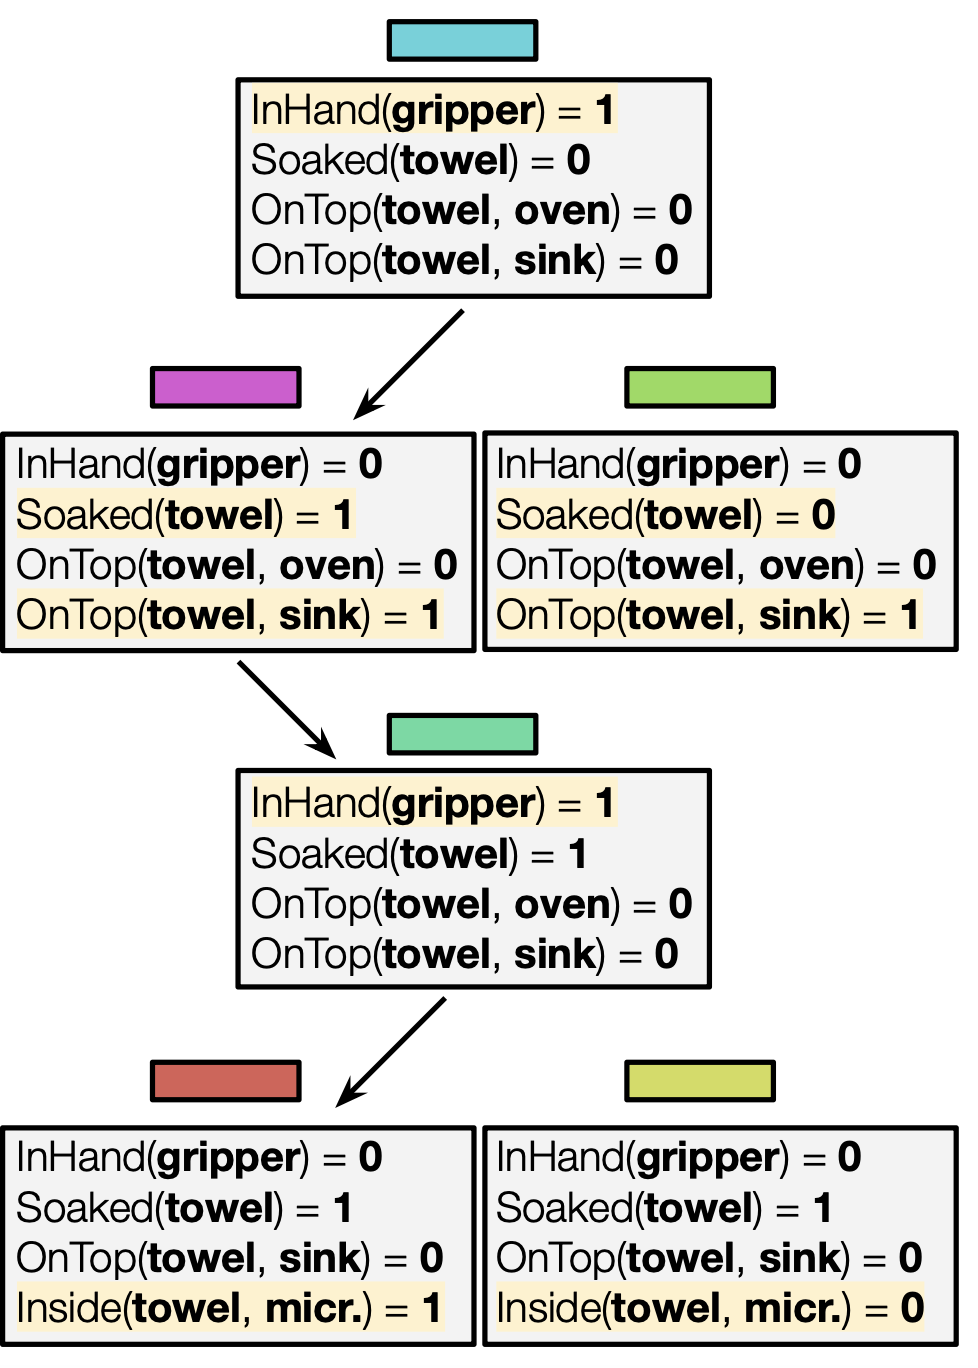
\includegraphics[width=0.5\textwidth]{figures/bfs_predicates.png}
	\caption{Caption describing your figure.}
	\label{fig:bfspredicates}
  \end{figure}
  

\subsection{Skills and Predicate Learning}

Consider the robot's joint states as \(q \in Q\) and the camera observation as \(o \in O\). Each of the actions in the task planning corresponds
to a skill \(s \in S\). Each skill has a corresponding visuomotor policy \(\pi\) that is learned from expert demonstrations. The policy predicts the
next state \(q\) for the robot given an observation \(o\). Given a sequence of states and observations in an expert trajectory \(\{(q_t, o_t)\}^T_{t=0}\),the
skill is trained to predict a state \(q_{t+1}\) for an observation \(o_t\). Each skill also has a termination policiy that outputs a binary value indicating
if the skill has been completed. The termination policy is trained to predict the termination condition of the skill. 

\subsection{Learning Transition Model}
Another challenge of task planning is to predict the effects of skills so that the robot could determine the best skill plan to reach a goal. For simplicity
purposes the Transition Model (Effects on the environment for a given skill) gave been hardcoded, however transition models could also be learned. Generalizable
transition models are subject to further research, as creating a model that can predict the effects of a skill on the environment is a challenging task given the specific
effect of skills under certain environments.


\begin{table}
	\caption{Learned Skills and Predicates.}
	\centering
	\begin{tabular}{l l r}
		\toprule
		\cmidrule(r){1-2}
		Name & Description & Type \\
		\midrule
		ReachOnTable & Reach object & Skill \\
		ReachOnTower & Reach object & Skill \\
		Stack & Stack object & Skill \\
		On & On Top & Predicate \\
		InHand & In Hand & Predicate \\
		\bottomrule
	\end{tabular}
	\label{tab:distcounts}
\end{table}

%------------------------------------------------

\section{Results}

\subsection{Proposed Architecture}
For learned skills, termination conditions and the predicated the model architecture will take as an input a point cloud image of the scene.
The point cloud is processed to generate a segmentation mask of the scene that will highlight objects of interest to a particular task. For 
example for the skill \(\verb|ReachOnTable|\) the model will generate a segmentation mask that highlights the object that the robot needs to reach.
Then  a PointNet++ architecture is used to extract the object-level features from the segmentation mask. The point cloud features are appended with
the features extracted from the joint states of the arm to predict either the joint targets, in the case of the skills, or the probability of a given
skill being terminated. The skills are trained with a linear combination of joint-space and operations loss, meanwhile the termination policies are trained
with a binary cross-entropy loss.

\par
\textbf{Joint-space loss}
The joint-space loss is the mean squared error between the predicted joint targets and the ground truth joint targets. The joint targets are the joint
angles that the robot needs to reach in order to execute a skill. The joint-space loss is defined as follows:
\begin{equation}
	L = \frac{1}{n} \sum_{i=1}^{n} (y_{\text{true},i} - y_{\text{pred},i})^2
\end{equation}

\par
\textbf{Operation loss}
The operation loss is used to minimize the loss to the final Cartesian end-effector position. The end-effector is represented with two points, one on the
x and y axis. These two points determine the robots end-effector position. Using forward kinematics, the joint state \(q\) is mapped for the prediction and the
ground truth. The operation loss is defined as follows:
\begin{equation}
	p_{\text{true},i} = f(q_{\text{true},i})
\end{equation}
	
\begin{equation}
	p_{\text{pred},i} = f(q_{\text{pred},i})
\end{equation}
	
\begin{equation}
	L_{\text{op}} = \frac{1}{n} \sum_{i=1}^{n} (p_{\text{true},i} - p_{\text{pred},i})^2
\end{equation}


\subsection{Task Planning and Execution}
The goal is defined by a list of predicates \(L_g\). A set of predicates \(p \in P\) is used to generate a logical state of the environment. The task planner finds a
sequence of skills from the set of Skills \(S\) that will satisfy the goal. The task planner uses a breadth-first search to find the optimal sequence of skills. 
The search algorithm takes a pair of start and goal state and generates a sequence of skills that will transform the start state into the goal state. The logical effects
of skills are updated after each skill is executed. The preconditions of the next skill are updated based on the logical effects of the previous skill. The search algorithm
continues until the goal is satisfied. The following algorithm describes the task planning algorithm:
\begin{algorithm}
	\caption{Execution}
	\begin{algorithmic}[1]
	\Procedure{Execute}{$L_G$}
		\State $replan\_counter \gets 0$
		\While{$replan\_counter < MAX\_REPLANS$}
			\State $o \gets \textsc{Observe}()$
			\State $P \gets \textsc{Plan}(o, L_G)$
			\State $replan\_counter \gets replan\_counter + 1$
			\If{$\textsc{ExecutePlan}(o, L_G, P) = \text{Success}$}
				\State \Return Success
			\EndIf
		\EndWhile
		\State \Return Failure
	\EndProcedure
	
	\Procedure{ExecutePlan}{$o, L_G, P$}
		\State $i \gets 0$
		\While{$i < |P|$}
			\State $s \gets P_i$
			\While{not $\forall p \in L_P, p(o) = \text{True}$}
				\State $i \gets i - 1$
				\If{$i < 0$}
					\State \Return Failure
				\EndIf
				\State $s \gets P_i$
			\EndWhile
			\State $retrial\_counter[s] \gets retrial\_counter[s] + 1$
			\If{$retrial\_counter[s] > MAX\_RETRIALS$}
				\State \Return Failure
			\EndIf
			\State $\textsc{ExecuteSkill}(s)$
			\State $o \gets \textsc{Observe}()$
			\If{$\forall p \in L_G, p(o) = \text{True}$}
				\State \Return Success
			\EndIf
			\State $i \gets i + 1$
		\EndWhile
		\State \Return Failure
	\EndProcedure
\end{algorithmic}
\end{algorithm}	

\begin{figure}[htb]
	\centering
	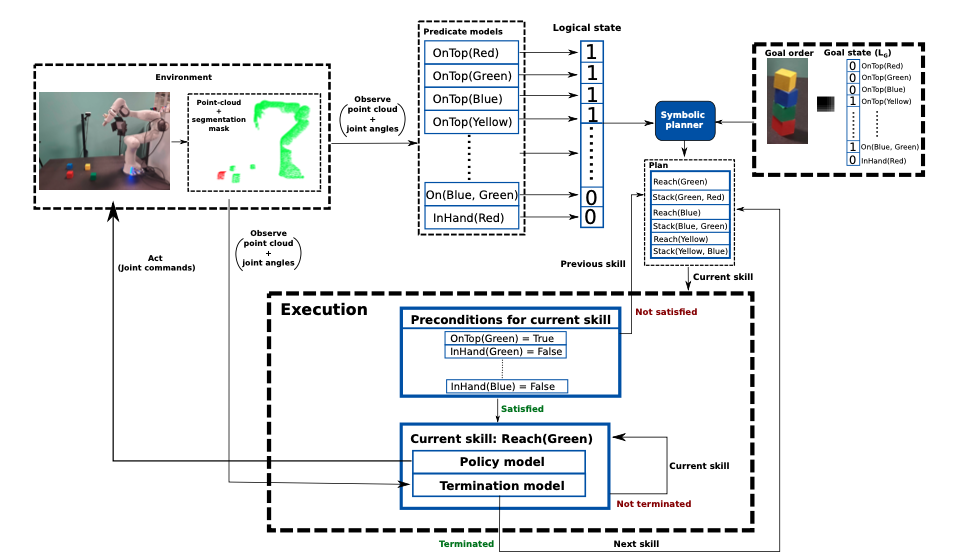
\includegraphics[width=0.5\textwidth]{figures/arch_diagram.png}
	\caption{Overview of model architecture.}
	\label{fig:archdiagram}
  \end{figure}
  
An example of the execution of the algorithm is shown in the following figure.
\par
Initial predicates:
\begin{align*}
    \text{on-table}(red) & : \text{False} \\
    \text{in-hand}(red) & : \text{False} \\
    \text{on-top}(red, blue) & : \text{False} \\
    \text{on-top}(red, green) & : \text{False} \\
    \text{on-table}(blue) & : \text{False} \\
    \text{in-hand}(blue) & : \text{False} \\
    \text{on-top}(blue, red) & : \text{False} \\
    \text{on-top}(blue, green) & : \text{False} \\
    \text{on-table}(green) & : \text{False} \\
    \text{in-hand}(green) & : \text{False} \\
    \text{on-top}(green, red) & : \text{False} \\
    \text{on-top}(green, blue) & : \text{False}
\end{align*}

Goal predicates:
\begin{align*}
    \text{on-top}(red, blue) & : \text{True}
\end{align*}

Plan:
\begin{enumerate}
    \item reach-on-table(red)
    \item stack(red, blue)
\end{enumerate}

Github repository: \url{https://github.com/miguel-merlin/generalizable_task_planning}\



%----------------------------------------------------------------------------------------
%	 REFERENCES
%----------------------------------------------------------------------------------------

% \printbibliography % Output the bibliography

%----------------------------------------------------------------------------------------

\end{document}
